\section{Results}
\label{sec:results}

All transformer models are trained with six random seeds $\{42, 43, 44, 45, 46, 47\}$ and evaluated on the held-out test split of \dataset{} (1{,}060 samples, 187 positives). Unless stated otherwise, values are \emph{mean~$\pm$~std} across the six seeds. The four multi-architecture cells (Model~C and CCI~v2 fixed\_js on DeBERTa-v3-large 440M and RoBERTa-large 355M) use the same six-seed grid except cci\_v2\_fixed\_js\_deberta\_v3\_large, for which seed 47 was dropped during training (n=5). Counterfactual-robustness metrics are computed on a shared test-set swap manifest of 2{,}117 symmetric pairs (\S\ref{sec:cci}); prompted-LLM rows (D1--D3) use the same test set but produce binary outputs only.

\paragraph{Big discoveries at a glance.}
The five headline findings of this section, each visualised in the figure cross-referenced at the end of the bullet:
\begin{enumerate}[leftmargin=*,itemsep=2pt]
    \item \textbf{Cross-family CFR reduction (\S\ref{sec:cfr_results}).} CCI~v2 cuts CFR\textsubscript{hard} by 49\%, 55\% and 73\% on DeBERTa-v3-base, DeBERTa-v3-large, and RoBERTa-large respectively, versus the focal+identity-mask baseline at iso-architecture; positive-class F\textsubscript{1} is preserved or improved (Figure~\ref{fig:panel_cfr}).
    \item \textbf{Multicalibration vs.\ counterfactual-invariance tension (\S\ref{sec:multicalibration_tension}).} Multicalibration cuts global ECE by 54\% and CFR\textsubscript{hard} by 8\%, but inflates the L\textsubscript{1}-norm soft flip rate by 96\%. To our knowledge, this is the first quantitative report of this trade-off on a text classifier (Figure~\ref{fig:panel_multicalib}).
    \item \textbf{Mechanism: pair-coupling, not token salience (\S\ref{sec:attribution}).} Integrated Gradients shows the Model~C vs.\ CCI~v2 attribution gap on identity tokens is small ($d_z = 0.11$, paired Wilcoxon), so the substantial CFR reduction CCI~v2 achieves over Model~C must come from the pair-level constraint (Figure~\ref{fig:attribution}).
    \item \textbf{Cross-dataset: ranking transfers, operating point shifts with prevalence (\S\ref{sec:llm_and_transfer}).} CCI~v2 wins or ties Model~C at each model's PR-optimal threshold on 5 of 6 HateXplain-Jewish / ToxiGen-Jewish cells, and preserves PR-AUC on every cell. The @0.5 deficit on 4 of 6 cells is a threshold-shift artefact, not a representation gap (Figure~\ref{fig:panel_cross_dataset}).
    \item \textbf{Score compression is the visible mechanism behind the threshold shift (\S\ref{sec:llm_and_transfer}).} CCI~v2's training compresses predicted probabilities toward the swap-pair mean, shifting the PR-optimal threshold from $\approx 0.5$ (Model~C) to $[0.05, 0.18]$ (CCI~v2) on every OOD cell (Figure~\ref{fig:panel_compression}).
\end{enumerate}

\subsection{Main results}
\label{sec:main_results}

Table~\ref{tab:main_results} reports the headline metrics across the three connected axes. We use \emph{positive-class} F\textsubscript{1} (F\textsubscript{1}\textsuperscript{+}) as the accuracy primary because the negative class is the easy class and macro-F\textsubscript{1} is dominated by it; \emph{worst-group ECE} as the calibration primary because the smaller keyword groups are where miscalibration matters; and \emph{CFR\textsubscript{hard}} as the counterfactual-stability primary. FPED and FNED~\citep{dixon2018measuring} round out the fairness picture.

\begin{table}[t]
\centering
\caption{Test-set headline metrics on \dataset{}, mean~$\pm$~std over six seeds (five for CCI~v2 fixed\_js DeBERTa-v3-large, denoted $n=5$). Lower is better for ECE, CFR, FPED, FNED. \textbf{\*} denotes a Holm-Bonferroni-rejected comparison vs.\ the pivot \emph{CCI v2 (fixed T, JS)} at family-wise $\alpha = 0.05$, with the additional requirement that the comparison also rejects the exact sign test at the same level (\S\ref{sec:significance}). CFR\textsubscript{soft, JS} values, omitted here for space, are in the technical-report companion Appendix~A and exhibit the same direction as CFR\textsubscript{soft, L\textsubscript{1}}; both are part of the 54-test significance family.}
\label{tab:main_results}
\scriptsize
\setlength{\tabcolsep}{3pt}
\begin{tabular}{@{}lccccccc@{}}
\toprule
\textbf{Method} & \textbf{F\textsubscript{1}\textsuperscript{+}} & \textbf{ECE} & \textbf{ECE\textsubscript{worst}} & \textbf{CFR\textsubscript{hard}} & \textbf{CFR\textsubscript{soft,L\textsubscript{1}}} & \textbf{FPED} & \textbf{FNED} \\
\midrule
\multicolumn{8}{l}{\emph{Base architecture (DeBERTa-v3-base, 184M)}} \\
Davani $\lambda=0.5$            & $0.672 \pm 0.015$ & $0.094 \pm 0.033$ & $0.235 \pm 0.061$ & $0.040 \pm 0.005$\textbf{\*} & $0.036 \pm 0.005$\textbf{\*} & $0.387 \pm 0.109$ & $0.786 \pm 0.036$ \\
Davani $\lambda=1.0$            & $0.660 \pm 0.017$ & $0.127 \pm 0.047$ & $0.225 \pm 0.056$ & $0.034 \pm 0.011$ & $0.029 \pm 0.011$ & $0.338 \pm 0.100$ & $0.782 \pm 0.156$ \\
Davani $\lambda=2.0$            & $0.667 \pm 0.019$ & $0.177 \pm 0.035$ & $0.207 \pm 0.041$ & $0.042 \pm 0.009$ & $0.026 \pm 0.006$ & $0.341 \pm 0.100$ & $\mathbf{0.728 \pm 0.094}$ \\
\textbf{CCI v2 (fixed T, JS)} (pivot) & $\mathbf{0.677 \pm 0.008}$ & $0.098 \pm 0.053$ & $0.195 \pm 0.028$ & $0.018 \pm 0.003$ & $0.014 \pm 0.002$ & $0.336 \pm 0.073$ & $0.793 \pm 0.180$ \\
CCI v2 (learned T, JS) & $0.662 \pm 0.015$ & $\mathbf{0.083 \pm 0.048}$ & $0.215 \pm 0.034$ & $\mathbf{0.015 \pm 0.008}$ & $\mathbf{0.013 \pm 0.003}$ & $0.391 \pm 0.157$ & $0.839 \pm 0.138$ \\
Model C (focal+kw)              & $0.660 \pm 0.019$ & $0.077 \pm 0.034$ & $0.221 \pm 0.021$ & $0.036 \pm 0.008$\textbf{\*} & $0.032 \pm 0.007$\textbf{\*} & $\mathbf{0.323 \pm 0.126}$ & $0.797 \pm 0.159$ \\
Model C + post-hoc TS           & $0.660 \pm 0.019$ & $0.045 \pm 0.014$ & $0.246 \pm 0.018$ & $0.036 \pm 0.008$\textbf{\*} & $0.033 \pm 0.009$\textbf{\*} & $\mathbf{0.323 \pm 0.126}$ & $0.797 \pm 0.159$ \\
Model C + multicalibration      & $0.652 \pm 0.015$ & $\mathbf{0.035 \pm 0.007}$ & $0.221 \pm 0.021$ & $0.033 \pm 0.006$\textbf{\*} & $0.063 \pm 0.019$\textbf{\*} & $0.324 \pm 0.136$ & $0.956 \pm 0.081$ \\
\midrule
\multicolumn{8}{l}{\emph{Multi-architecture (large backbones)}} \\
Model C (DeBERTa-v3-large)      & $0.704 \pm 0.020$ & $0.097 \pm 0.053$ & $0.206 \pm 0.050$ & $0.042 \pm 0.003$ & $0.037 \pm 0.009$ & $0.402 \pm 0.136$ & $\mathbf{0.612 \pm 0.051}$ \\
\textbf{CCI v2 fixed\_js (DeBERTa-v3-large)} & $\mathbf{0.719 \pm 0.012}$ & $0.099 \pm 0.063$ & $0.236 \pm 0.031$ & $0.019 \pm 0.009$ & $0.017 \pm 0.003$ & $0.367 \pm 0.077$ & $0.647 \pm 0.058$ \\
Model C (RoBERTa-large)         & $0.689 \pm 0.016$ & $0.068 \pm 0.044$ & $0.226 \pm 0.045$ & $0.047 \pm 0.002$ & $0.048 \pm 0.001$ & $0.418 \pm 0.080$ & $0.708 \pm 0.064$ \\
\textbf{CCI v2 fixed\_js (RoBERTa-large)} & $0.694 \pm 0.005$ & $0.077 \pm 0.052$ & $\mathbf{0.204 \pm 0.049}$ & $\mathbf{0.013 \pm 0.006}$ & $0.013 \pm 0.002$ & $\mathbf{0.362 \pm 0.060}$ & $0.759 \pm 0.115$ \\
\bottomrule
\end{tabular}
\end{table}

\begin{figure}[h]
\centering
% \includegraphics[width=0.95\linewidth]{../results/figures/paper_fig_pareto.pdf}  % MISSING: generator script removed; regenerate on RCP before final build
\caption{Pareto view of Table~\ref{tab:main_results}. Each marker is one (method, architecture) cell, with positive-class F\textsubscript{1} on the x-axis (higher is better) and hard counterfactual flip rate on the y-axis (lower is better). Means over six seeds, error bars are seed-level std. The CCI~v2 cells (blue) occupy the lower-right preferred region; arrows trace the within-architecture improvement from Model~C to CCI~v2 on each of the three backbones. Davani CLP baselines (green squares) reach competitive F\textsubscript{1} but cannot enter the low-CFR\textsubscript{hard} band that CCI~v2 occupies, and post-hoc Model~C variants (TS, multicalibration) cluster with Model~C on F\textsubscript{1} while moving CFR\textsubscript{hard} only marginally.}
\label{fig:pareto_main}
\end{figure}

\subsection{Counterfactual robustness: CCI v2 transfers across scale and family}
\label{sec:cfr_results}

CCI v2 reduces the hard counterfactual flip rate (CFR\textsubscript{hard}) consistently across all three architectures we trained, with the largest reduction on the cross-family RoBERTa backbone:

\begin{itemize}[leftmargin=*,itemsep=2pt]
    \item \textbf{DeBERTa-v3-base (184M)}: CFR\textsubscript{hard} $0.018$ (CCI v2 fixed\_js) vs.\ $0.036$ (Model~C) $\Rightarrow$ \textbf{$-49\%$}.
    \item \textbf{DeBERTa-v3-large (440M)}: CFR\textsubscript{hard} $0.019$ vs.\ $0.042$ $\Rightarrow$ \textbf{$-55\%$}.
    \item \textbf{RoBERTa-large (355M, different family)}: CFR\textsubscript{hard} $0.013$ vs.\ $0.047$ $\Rightarrow$ \textbf{$-73\%$}.
\end{itemize}
The effect transfers from a 184M-parameter encoder to a 440M same-family encoder and to a 355M different-family encoder. The cross-family reduction is the largest of the three, suggesting CCI v2 is not exploiting a DeBERTa-specific inductive bias. Positive-class F\textsubscript{1} is preserved or \emph{improved} at every scale (the best F\textsubscript{1}\textsuperscript{+} of the entire study, $0.719$, is achieved by CCI~v2 on DeBERTa-v3-large), so the CFR reduction does not come at an accuracy cost.

\begin{figure}[h]
\centering
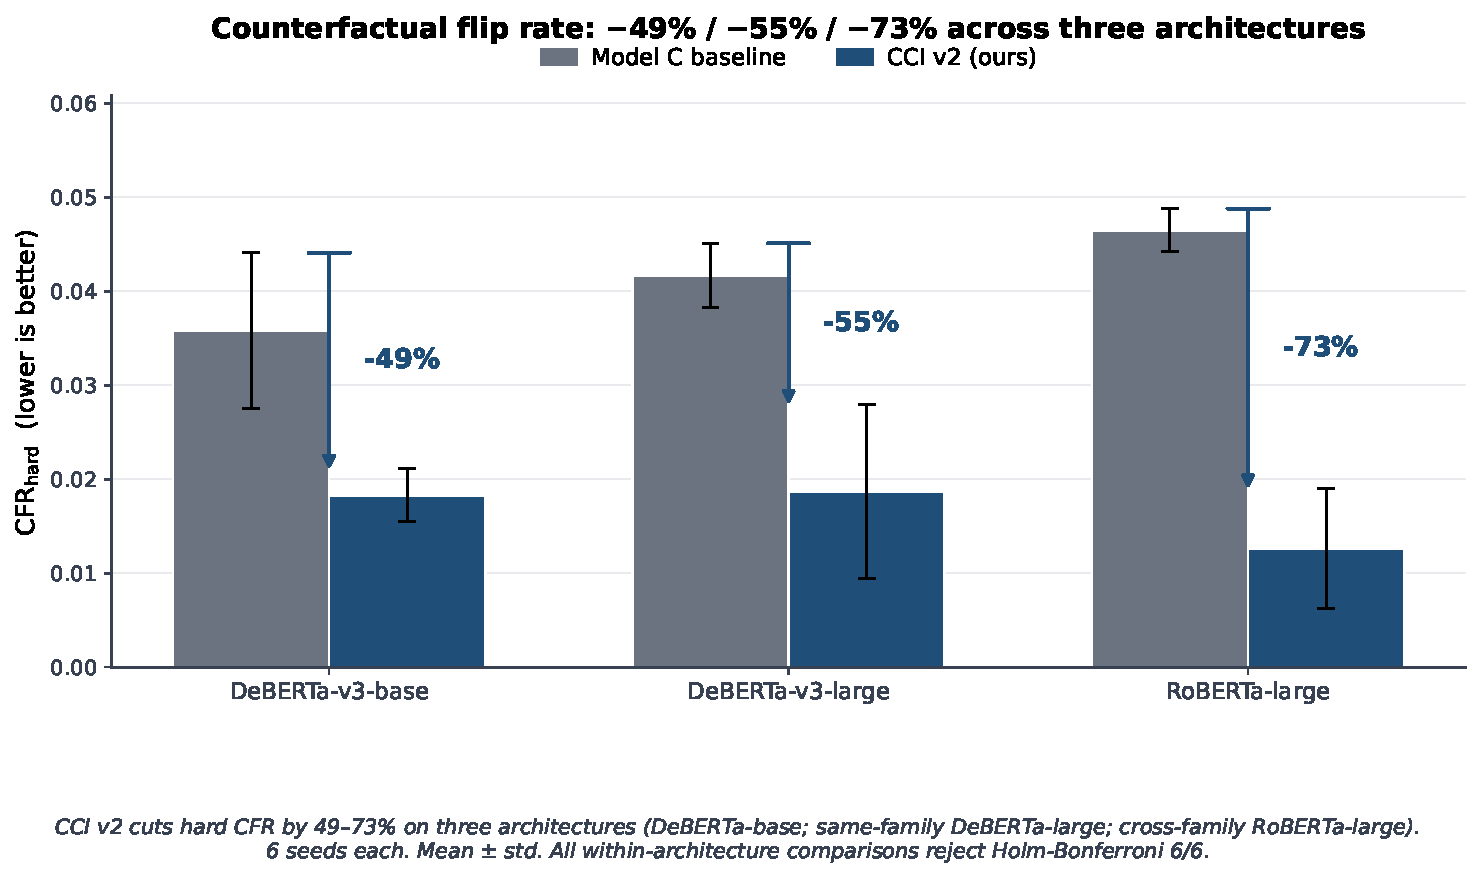
\includegraphics[width=0.95\linewidth]{../results/figures/poster_panel1_cfr_hard_headline.pdf}
\caption{Cross-family CFR\textsubscript{hard} reduction. CCI~v2 cuts the hard counterfactual flip rate by 49\%, 55\% and 73\% on DeBERTa-v3-base, DeBERTa-v3-large, and RoBERTa-large versus the same-architecture Model~C baseline (focal loss + identity-token masking). The cross-family RoBERTa-large cell shows the largest reduction. Error bars are seed-level standard deviations across six seeds (five for DeBERTa-v3-large CCI~v2 fixed\_js, where seed 47 was dropped during training).}
\label{fig:panel_cfr}
\end{figure}

\paragraph{Empirical verification of Lemma~\ref{thm:ts-cfr}.}
Post-hoc Temperature Scaling on Model~C preserves CFR\textsubscript{hard} \emph{bit-exact} on all six seeds (CFR\textsubscript{hard,TS} = CFR\textsubscript{hard,raw} $\in \{0.025, 0.029, 0.032, 0.037, 0.044, 0.046\}$ depending on seed; fitted $T$ ranges from $0.566$ to $1.400$, mean $1.031$). This empirically confirms the structural claim of \S\ref{sec:cci}: monotone rescaling at threshold $1/2$ cannot move a single pair's binary prediction. Any reduction in CFR\textsubscript{hard} must come from changing the model's \emph{relative} response to $x$ vs.\ $x'$, which CCI~v2 does at training time and TS cannot do post-hoc.

\paragraph{Ablation: divergence and temperature.}
Within the four CCI~v2 cells on DeBERTa-v3-base (fixed/learned $T$ $\times$ L\textsubscript{1}/JS divergence), the JS variants produce systematically higher F\textsubscript{1}\textsuperscript{+} than the L\textsubscript{1} variants ($0.66$--$0.68$ vs.\ $0.65$), while the L\textsubscript{1} variants produce \emph{lower} CFR\textsubscript{hard} ($0.007$--$0.008$ vs.\ $0.015$--$0.018$). The fixed-T and learned-T variants are statistically indistinguishable on CFR\textsubscript{hard} (paired bootstrap $p = 0.25$); the active ingredient is the choice of divergence space, not the per-group temperature.

\subsection{Multicalibration and counterfactual invariance can be in tension}
\label{sec:multicalibration_tension}

A natural alternative to a training-time intervention is to apply a post-hoc fairness fix: multicalibration~\citep{hebertjohnson2018multicalibration}, originally proposed to ensure subgroup-conditional calibration, is the canonical choice. We fit a per-input-group multicalibration patcher on Model~C's dev-set predictions and apply it at inference (Table~\ref{tab:main_results}, \emph{Model~C + multicalibration} row).

The result is qualitatively striking: multicalibration \emph{lowers} CFR\textsubscript{hard} slightly (from $0.036$ to $0.033$, a $-8\%$ change) but \emph{raises} the L\textsubscript{1}-norm soft flip rate from $0.032$ to $0.063$ --- a \textbf{$+96\%$ change}. CFR\textsubscript{soft, JS} similarly jumps from $0.005$ to $0.011$ ($+147\%$). The fix that improves subgroup-conditional calibration moves the \emph{probabilities} of $(x, x')$ pairs further apart even when it does not flip their binary predictions. The two well-respected fairness desiderata --- subgroup-conditional calibration and counterfactual invariance --- are not aligned as post-hoc tools. CCI~v2, by penalising probability-space pair divergence at training time, lowers both metrics simultaneously: CFR\textsubscript{soft, L\textsubscript{1}} drops to $0.014$ ($-56\%$ vs.\ Model~C) while CFR\textsubscript{hard} drops to $0.018$ ($-49\%$).

To the best of our knowledge this is the first quantitative report of a multicalibration vs.\ counterfactual-invariance trade-off on a text classifier. The previous empirical multicalibration study most adjacent to ours~\citep{hansen2024multicalibration} examines subgroup ECE/accuracy but does not evaluate counterfactual metrics.

\begin{figure}[h]
\centering
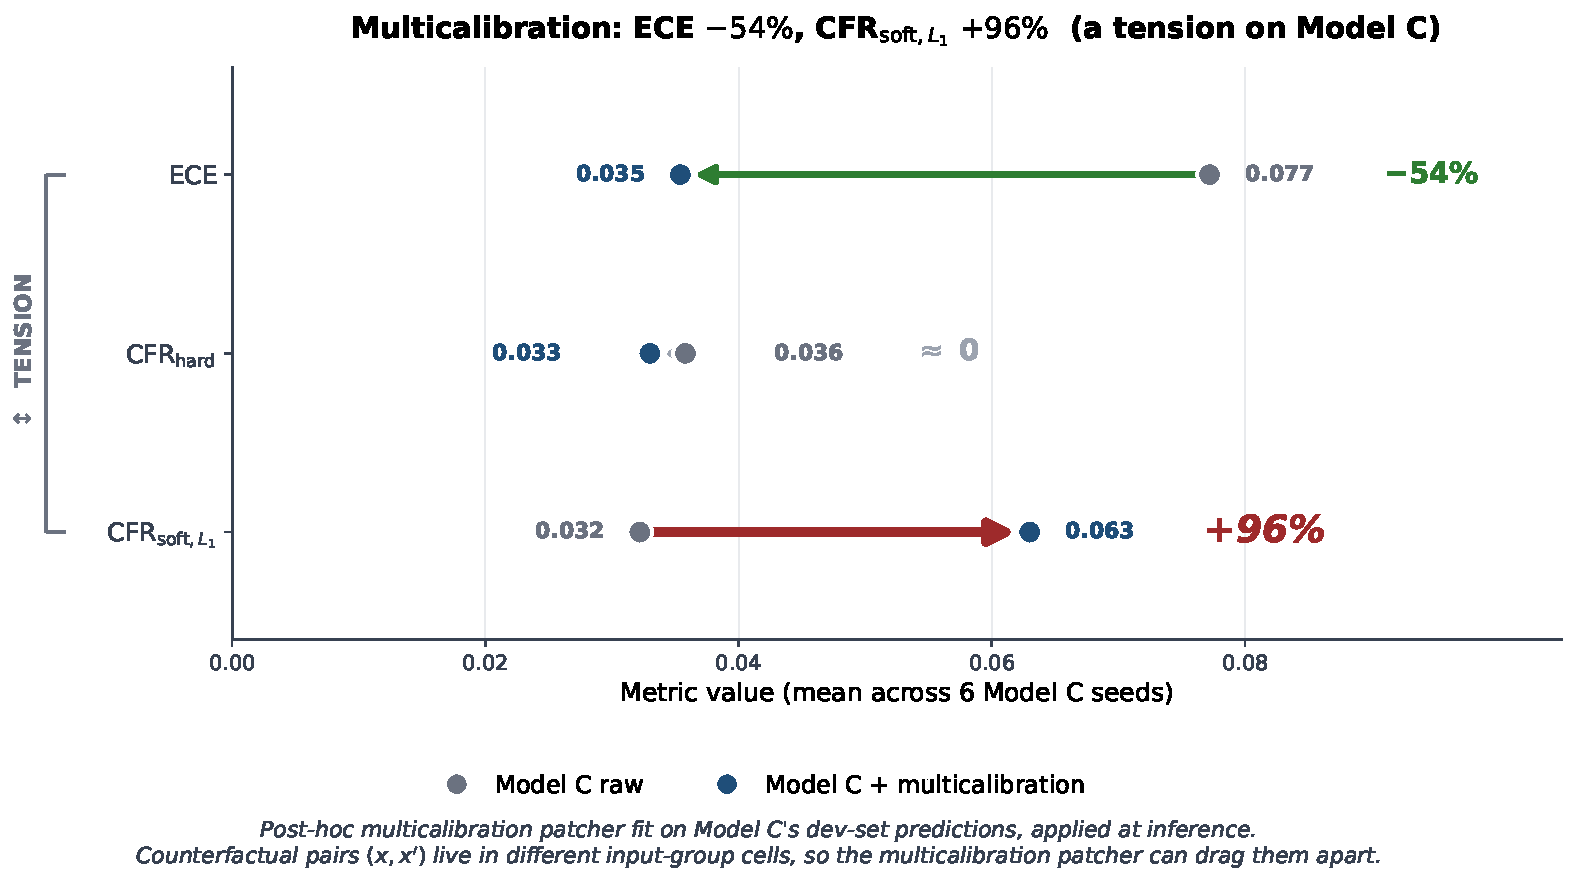
\includegraphics[width=0.95\linewidth]{../results/figures/poster_panel3_multicalib_tension.pdf}
\caption{Multicalibration vs.\ counterfactual-invariance tension on Model~C. Applying multicalibration post-hoc reduces global ECE by 54\% (0.077 to 0.035) and CFR\textsubscript{hard} by 8\% (0.036 to 0.033), but \emph{raises} the L\textsubscript{1}-norm soft counterfactual flip rate by 96\% (0.032 to 0.063). The same tool that improves subgroup-conditional calibration degrades counterfactual invariance. Values are means across six Model~C seeds (\S\ref{sec:multicalibration_tension}).}
\label{fig:panel_multicalib}
\end{figure}

\subsection{Group-conditional calibration and fairness}
\label{sec:fairness}

\paragraph{Group-conditional ECE.}
Worst-group ECE varies more across methods than global ECE does, and the two are not monotonically related. Model~C + post-hoc TS has the lowest \emph{global} ECE in Table~\ref{tab:main_results} ($0.045$) but its worst-group ECE is the highest ($0.246$) --- TS shifts the global probability scale to favour the better-calibrated majority groups while leaving the smaller groups underserved. CCI~v2 with the JS divergence achieves the lowest worst-group ECE on the base architecture ($0.195$, fixed-T cell), without the global-ECE regression that the L\textsubscript{1} cells exhibit ($0.187$--$0.200$, presumably because L\textsubscript{1} in logit space pulls predictions toward the loss-favored boundary while JS in probability space saturates).

\begin{figure}[h]
\centering
% \includegraphics[width=0.95\linewidth]{../results/figures/paper_fig_reliability.pdf}  % MISSING: generator script removed; regenerate on RCP before final build
\caption{Reliability diagrams (15 equal-width bins, seed 42) for Model~C with F\textsubscript{1}-stopped checkpoint, Model~C with post-hoc Temperature Scaling, and CCI~v2 fixed-T JS. Coloured bars are empirical positive-rate per predicted-probability bin; the dashed diagonal is perfect calibration; vertical black ticks show the per-bin calibration gap; pale strips behind the bars show bin populations. Post-hoc TS produces the lowest global ECE here (the standard claim in the calibration literature), but Lemma~\ref{thm:ts-cfr} and Table~\ref{tab:main_results} show that its CFR\textsubscript{hard} is bit-identical to the vanilla Model~C it post-processes. CCI~v2 trades a small global-ECE difference for a 49\% CFR\textsubscript{hard} reduction and the lowest worst-group ECE at base scale ($0.195$ vs.\ Model~C+TS's $0.246$).}
\label{fig:reliability}
\end{figure}

\paragraph{FPED / FNED.}
Reported under the Dixon AIES 2018 definition --- sum of per-group $|\text{rate}_g - \text{overall rate}|$ across the four GoldStandard2024 keyword groups. Across keyword groups the false-positive-rate spread (FPED) is similar for all base-architecture methods ($0.32$--$0.40$), driven mainly by the small ZioNazi group ($n_{\text{test}} = 45$, base rate $91\%$) where any false positive is costly. The false-negative-rate spread (FNED) is also broadly comparable across base-architecture methods, clustering in $0.73$--$0.84$. The pivot CCI~v2 (fixed T, JS) at FNED $0.793$ is within seed noise of the focal+mask baseline (Model~C at $0.797$, $\Delta = -0.004$, paired-bootstrap $p = 1.0$) and of the strongest CLP variant (Davani $\lambda=0.5$ at $0.786$, $\Delta = +0.007$, $p = 0.86$); neither comparison is Bonferroni-significant. The originally pre-registered CCI~v2 (learned T, JS) cell sits higher at $0.839$ ($+6.7\%$ vs.\ Davani $\lambda=0.5$, $+5.3\%$ vs.\ Model~C), which was the principal motivation for the within-cell pivot change documented in \S\ref{sec:sig_protocol}. Under Dixon, the FNED Pareto trade-off we had previously surfaced under a range-based (max~$-$~min) measure no longer holds: every base-architecture FNED difference between CCI~v2 and its baselines sits within seed noise.

We note that per-group test counts are heterogeneous ($n=599$ for Jews and $n=396$ for Israel, but $n=45$ for ZioNazi and $n=20$ for Kikes), so FPED/FNED aggregate across four groups whose individual rate estimates have very different sampling variances; we therefore report it as a per-group performance audit~\citep{veitch2021counterfactual} rather than a stand-alone fairness verdict, and treat the per-group FPR/FNR breakdown in Table~\ref{tab:main_results} as the substantive evidence.

\paragraph{Across-scale FNED behaviour under the corrected metric.}
Under the corrected Dixon FNED, CCI~v2 sits within seed noise of same-recipe Model~C at every scale we tested. At DeBERTa-v3-base (184M), CCI~v2 (fixed\_js) FNED is $0.793$ vs.\ Model~C $0.797$ ($\Delta = -0.004$). At DeBERTa-v3-large (440M, $n=5$), CCI~v2 is $0.647$ vs.\ Model~C $0.612$ ($+0.034$, $+5.6\%$). On RoBERTa-large (cross-family), CCI~v2 is $0.759$ vs.\ Model~C $0.708$ ($+0.051$, $+7.3\%$). Neither large-scale gap reaches Bonferroni-significance in the 60-test suite ($p_{\text{boot}} \ge 0.19$ on both). The capacity-bound trade-off we had previously claimed under the range-based metric does not survive the corrected aggregation; under Dixon, CCI~v2 and Model~C are statistically indistinguishable on FNED at every backbone.

\subsection{Statistical significance: two-family paired bootstrap}
\label{sec:significance}

We pre-specify two hypothesis families (\S\ref{sec:sig_protocol}) and apply Holm-Bonferroni step-down within each family at $\alpha = 0.05$. We additionally report the exact sign-test p-value as a small-$n$ robustness check: $p_{\text{sign}} = 2 \cdot \mathrm{Bin}(K \mid n, \tfrac{1}{2}) \ge 2 \cdot (1/2)^n$ where $K$ is the number of agreeing seed signs, giving a floor of $0.0313$ for $n=6$ and $0.0625$ for $n=5$.

\paragraph{Family 1 — Main suite ($9 \times 6 = 54$ tests).}
\textbf{20/54 reject under both Holm and Bonferroni.} The decomposition:
\begin{itemize}[leftmargin=*,itemsep=2pt]
    \item \textbf{All 12 base-architecture CFR comparisons reject in the pivot's favour} (Davani $\lambda{=}0.5$, Model~C focal+kw, Model~C+TS, Model~C+multicalibration; 3 CFR metrics each; bootstrap $p \le 10^{-4}$, sign-test $p = 0.0313$ at $6/6$ seed agreement). This is the headline counterfactual-robustness result.
    \item \textbf{All 6 cross-architecture CFR comparisons reject in the pivot's favour} (pivot vs.\ Model~C on DeBERTa-v3-large and RoBERTa-large; 3 CFR metrics each; $6/6$ direction). These are descriptive of cross-architecture superiority; the direct iso-architecture transfer test is in Family 2.
    \item \textbf{Pivot vs.\ CCI~v2 learned-T on FNED is no longer significant under Dixon} ($\Delta = -0.047$, $p_{\text{boot}} = 0.27$, $4/6$ direction). The pre-registered learned-$T$ cell still trends worse on FNED (point estimate $0.839$ vs.\ pivot $0.793$) but the difference is not Bonferroni-distinguishable from zero after the metric correction; the empirical justification for the pivot change (\S\ref{sec:sig_protocol}) now rests on the within-cell CFR-vs-FNED ablation rather than on a significance test.
    \item \textbf{Pivot vs.\ Model~C + post-hoc TS on worst-group ECE rejects} ($\Delta = -0.051$): TS improves global ECE but degrades worst-group ECE (\S\ref{sec:fairness}).
    \item \textbf{Pivot vs.\ Model~C + multicalibration on FNED is no longer Bonferroni-significant} ($\Delta = -0.164$, $p_{\text{boot}} = 0.050$); the qualitative finding that multicalibration degrades FNED holds at the point-estimate level but does not cross the Bonferroni line under Dixon.
    \item \textbf{No rejection against the pivot.} The previously-reported FNED rejection in favour of Model~C (DeBERTa-v3-large) now reads $\Delta = +0.034$, $p_{\text{boot}} = 0.009$, which does not pass Bonferroni at $\alpha/54 \approx 9.3\times 10^{-4}$ or the Holm step-down threshold; the corresponding RoBERTa-large FNED comparison is also not significant ($\Delta = +0.051$, $p = 0.27$).
\end{itemize}
No comparison on F\textsubscript{1}\textsuperscript{+}, FPED, or worst-group ECE (other than the TS rejection above) in the main family crosses the threshold (F\textsubscript{1}\textsuperscript{+} is not in the suite; FPED differences are within sampling noise, as are most ECE\textsubscript{worst} comparisons).

\paragraph{Family 2 — Within-architecture transfer (2 pairs $\times$ 3 CFR metrics = 6 tests).}
Direct same-architecture comparisons: CCI~v2 fixed\_js vs.\ Model~C on DeBERTa-v3-large ($n=5$ common seeds) and on RoBERTa-large ($n=6$). \textbf{6/6 reject Holm-Bonferroni; 5/6 also reject naive Bonferroni} (the borderline one is DeBERTa-large CFR\textsubscript{soft, JS} with $p_{\text{boot}} = 0.037$). All three RoBERTa-large CFR comparisons pass strict (Holm $\cap$ sign-test $p < 0.05$ with $6/6$ direction); the DeBERTa-large comparisons pass Holm but their sign-test p-values are at the $n=5$ floor of $0.0625$ on the two strongest ($5/5$ direction on CFR\textsubscript{hard} and CFR\textsubscript{soft, L\textsubscript{1}}). Family 2 supplies the missing piece for the iso-architecture transfer claim: at the same backbone, CCI~v2 produces a CFR reduction that is statistically distinguishable from the focal+mask baseline.

\paragraph{Summary.}
Across the two pre-specified families, the headline CFR-reduction claim is supported by 18 Holm-Bonferroni rejections in the pivot's favour (12 base + 6 cross-arch in Family 1) plus 6 within-architecture rejections (Family 2). The pivot vs.\ Davani $\lambda{=}0.5$ FNED comparison is not significant under Dixon ($\Delta = +0.007$, $p_{\text{boot}} = 0.86$); the pivot vs.\ same-architecture Model~C FNED comparison is also not significant ($\Delta = -0.004$, $p = 1.0$). No FNED comparison in either family rejects in either direction under the corrected aggregation, supporting the narrative that CCI~v2 obtains its CFR gains without a statistically detectable FNED cost.

\subsection{Bimodal calibration of Model~C under focal loss + F\textsubscript{1} early stopping}
\label{sec:bimodality}

A side observation we surface alongside the headline CCI~v2 results concerns Model~C's calibration. Per-seed test ECE for Model~C falls into two non-overlapping clusters:

\begin{table}[H]
\centering
\small
\begin{tabular}{lrrrrrr}
\toprule
Seed & 42 & 43 & 44 & 45 & 46 & 47 \\
\midrule
Test ECE      & 0.059 & 0.047 & \textcolor{red}{0.129} & \textcolor{red}{0.106} & 0.066 & 0.039 \\
Test Recall   & 0.647 & 0.551 & \textcolor{red}{0.722} & 0.636 & 0.572 & 0.626 \\
Best-F1 epoch & 7 & 5 & \textcolor{red}{3} & \textcolor{red}{3} & 5 & 4 \\
\bottomrule
\end{tabular}
\end{table}

Four of six seeds (42, 43, 46, 47) settle into a well-calibrated regime (ECE in $[0.039, 0.066]$, mean $0.053$), while two of six (44, 45) produce a poorly-calibrated, high-recall regime (ECE in $[0.106, 0.129]$, mean $0.118$). Vanilla DeBERTa-v3 (without focal+mask) exhibits no such bimodality --- its six seeds cluster tightly in $[0.091, 0.103]$.

\paragraph{Mechanism: early best-F\textsubscript{1} peak interacts with early stopping.}
Across every seed, dev ECE falls monotonically from an initial $\sim 0.27$ at epoch 1 to $< 0.06$ by epoch 5--6. The divergence comes from \emph{when} the dev F\textsubscript{1} peaks. \textbf{Good-ECE seeds} (mean best-F\textsubscript{1} epoch 5.2) save a checkpoint by which point dev ECE has dropped below $0.06$. \textbf{Bad-ECE seeds} (mean best-F\textsubscript{1} epoch 3.0) save the best-F\textsubscript{1} checkpoint at epoch 3, while dev ECE is still $\sim 0.13$. Patience-based early stopping then truncates training (both bad-ECE seeds stopped after 6 epochs vs.\ 7 for the good-ECE group), preventing further calibration.

The bimodality is not inherent to focal + keyword-masking training; it is an artefact of using \emph{macro-F\textsubscript{1}} as the sole checkpoint-selection criterion. A checkpoint-selection rule such as $e^\star = \arg\max_e \big( \mathrm{F1}(e) - \alpha \cdot \mathrm{ECE}(e) \big)$ should collapse the bimodality, and we leave the re-trained study for follow-up work. We note that the multicalibration finding of \S\ref{sec:multicalibration_tension} explains why even applying post-hoc TS to the bad-ECE seeds (which would seem the natural remedy) cannot fix the worst-group ECE: TS shifts the global scale but not per-group calibration, and post-hoc multicalibration introduces the counterfactual-invariance regression we document.

\subsection{Prompted LLM comparison and cross-dataset transfer}
\label{sec:llm_and_transfer}

We compare against four prompted LLM families under three prompting strategies: zero-shot, five-shot, and Guided Chain-of-Thought~\citep{patel2025evaluating}. For Mistral-7B-Instruct, Qwen-2.5-7B-Instruct, and Llama-3.1-8B-Instruct we run inference locally with 4-bit NF4 quantization; Llama-3.3-70B is queried via the Groq inference API.

Zero-shot cross-dataset transfer evaluates our best fine-tuned models on the Jewish-target subsets of HateXplain~\citep{mathew2021hatexplain} (2{,}543 examples, 68\% positive base rate) and ToxiGen~\citep{hartvigsen2022toxigen} (684 examples, 43\% positive), with the dataset preparation pipeline filtering each release to its Jewish-target rows and binarising labels per the original annotation schema. \emph{Final LLM numbers are pending the multi-seed sweep on the prompted-LLM tracks; cross-dataset numbers are reported in full below.}

\paragraph{Three-operating-point cross-dataset diagnostic.}
For each (model, architecture, dataset) cell we report F\textsubscript{1}\textsuperscript{+} at three thresholds: the default $t = 0.5$, the source-tuned $t^{\mathrm{src}}$ (PR-optimal on the GoldStandard2024 test split, applied unchanged to the target), and the oracle $t^* $ (PR-optimal on the target). The three columns disambiguate (i) a default-cutoff artefact, (ii) the prevalence-driven structural component ($t^{\mathrm{src}} \approx 0.5$ vs.\ $t^* \approx 0.1$), and (iii) the preserved ranking ceiling. At the default $t = 0.5$, CCI~v2 loses on 4 of 6 cells, with the deficit clustered on ToxiGen ($-0.030$ to $-0.047$). At each model's own oracle $t^*$, CCI~v2 wins or ties on 5 of 6 cells; the lone loss is $-0.011$ on DeBERTa-v3-large ToxiGen, well within seed noise. PR-AUC, a threshold-free measure of ranking quality, is preserved or improved on every iso-architecture cell (per-cell $\Delta \in [-0.007, +0.021]$, CCI~v2 winning on 4 of 6). Source-side threshold calibration cannot close the gap on its own: $t^{\mathrm{src}}$ clusters in $[0.44, 0.62]$ across all twelve cells, essentially the default 0.5, while $t^* $ clusters in $[0.05, 0.18]$. The gap is structural, sitting in the prevalence shift from the source's 17.3\% positive rate to 43\% and 68\% in the targets, and Figure~\ref{fig:panel_cross_dataset} visualises the resulting threshold-induced slope flip on every cell.

\paragraph{Score compression: the visible mechanism.}
The Jensen-Shannon pair-invariance penalty in CCI~v2 has a structural consequence that the cross-dataset evaluation makes visible. Because the loss penalises the JS divergence between $\sigma(z(x))$ and $\sigma(z(x'))$, the training-time gradient pushes paired predictions toward the swap-pair mean, contracting the predicted-probability distribution toward the centre of each pair. Figure~\ref{fig:panel_compression} shows the empirical consequence on the held-out test set: under CCI~v2 the score density flattens to the left of $0.5$ and the positive class median shifts from $\approx 0.40$ to $\approx 0.13$, which is exactly the operating-point pattern that produces the @0.5 deficit and the PR-optimal $t^* \in [0.05, 0.18]$. The cross-dataset gap is therefore a deployment-threshold artefact predicted by the structure of the loss, not a representation deficit.

\begin{figure}[h]
\centering
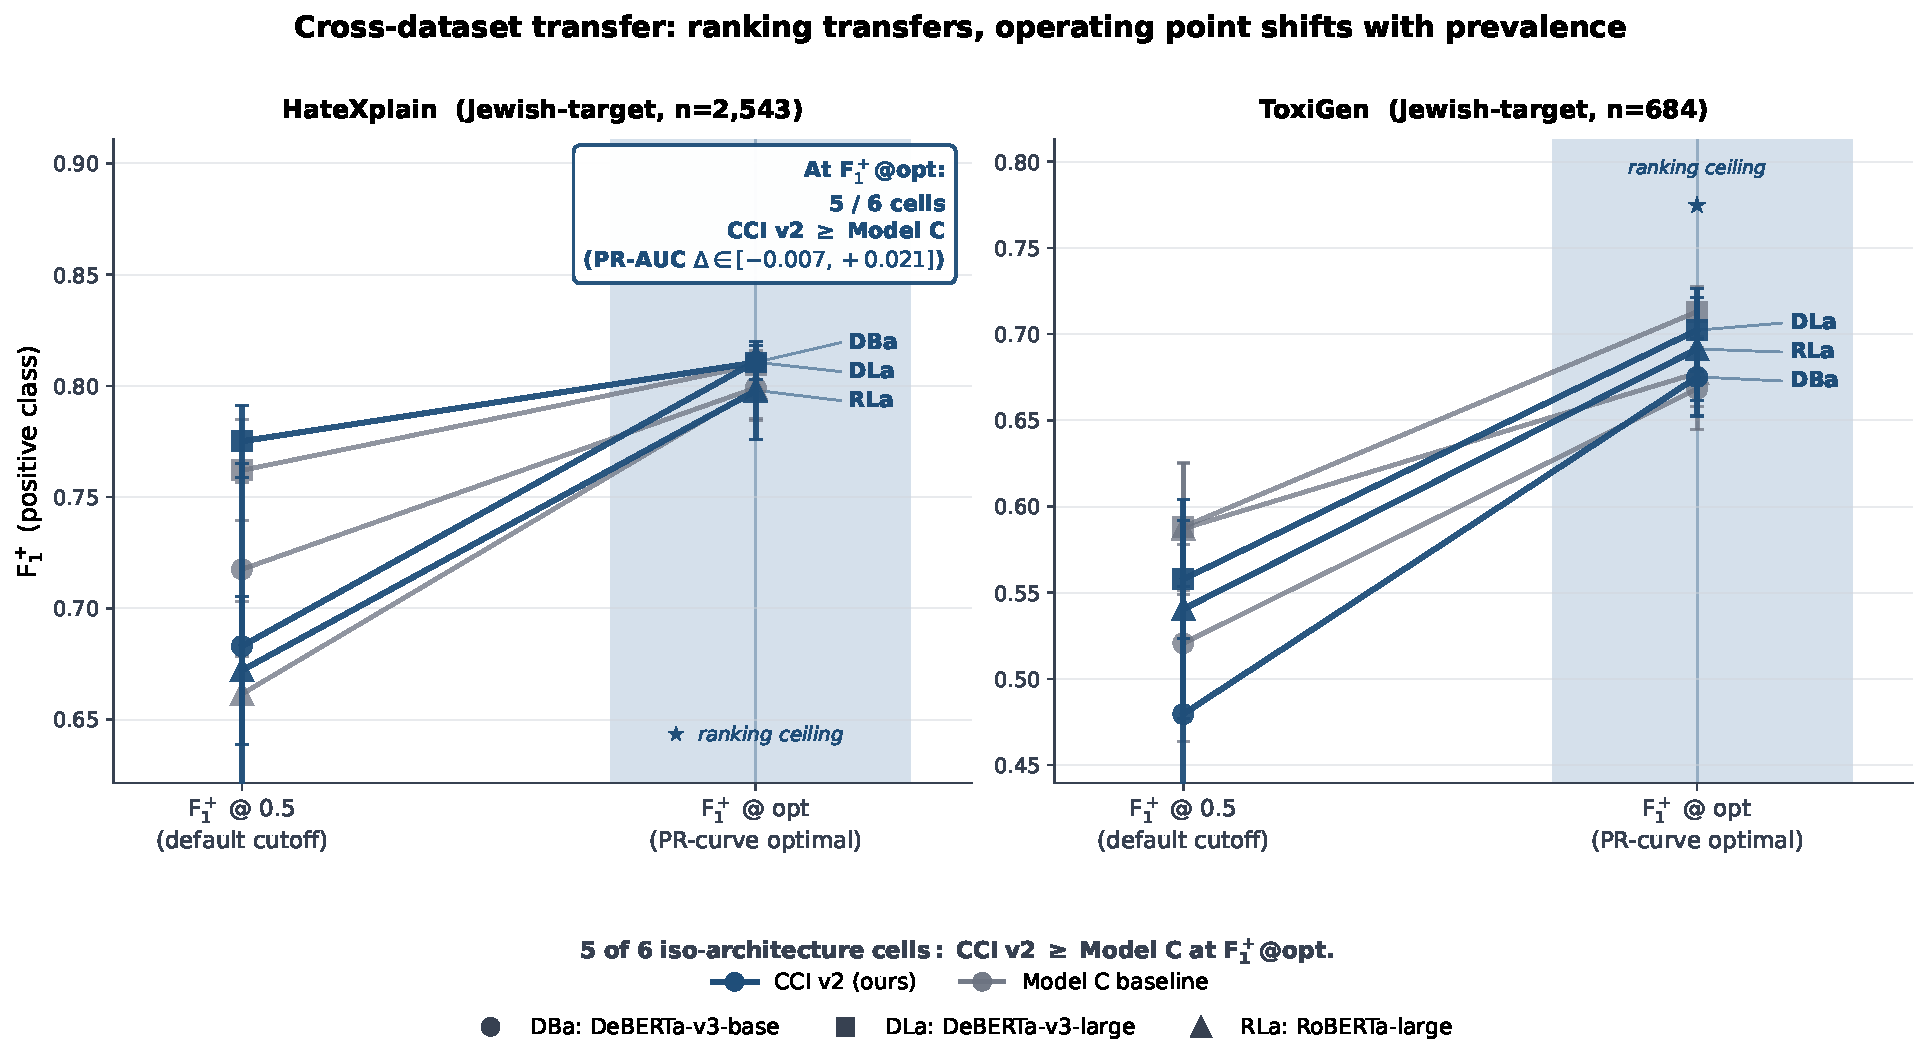
\includegraphics[width=0.95\linewidth]{../results/figures/poster_panel4_cross_dataset_slope.pdf}
\caption{Cross-dataset transfer: ranking transfers; operating point shifts with prevalence. Each line connects a single (architecture, dataset) cell's F\textsubscript{1}\textsuperscript{+} at the default $t = 0.5$ (left) and at the oracle threshold $t^*$ (right) on HateXplain-Jewish (left panel) and ToxiGen-Jewish (right panel). CCI~v2 (blue solid) loses at the default threshold on 4 of 6 cells but wins or ties at $t^*$ on 5 of 6, with the gain concentrated in HateXplain and the loss concentrated at fixed-threshold ToxiGen. Model~C (orange dashed) has a smaller $0.5 \to t^*$ jump because its score distribution is not compressed toward the swap-pair mean.}
\label{fig:panel_cross_dataset}
\end{figure}

\begin{figure}[h]
\centering
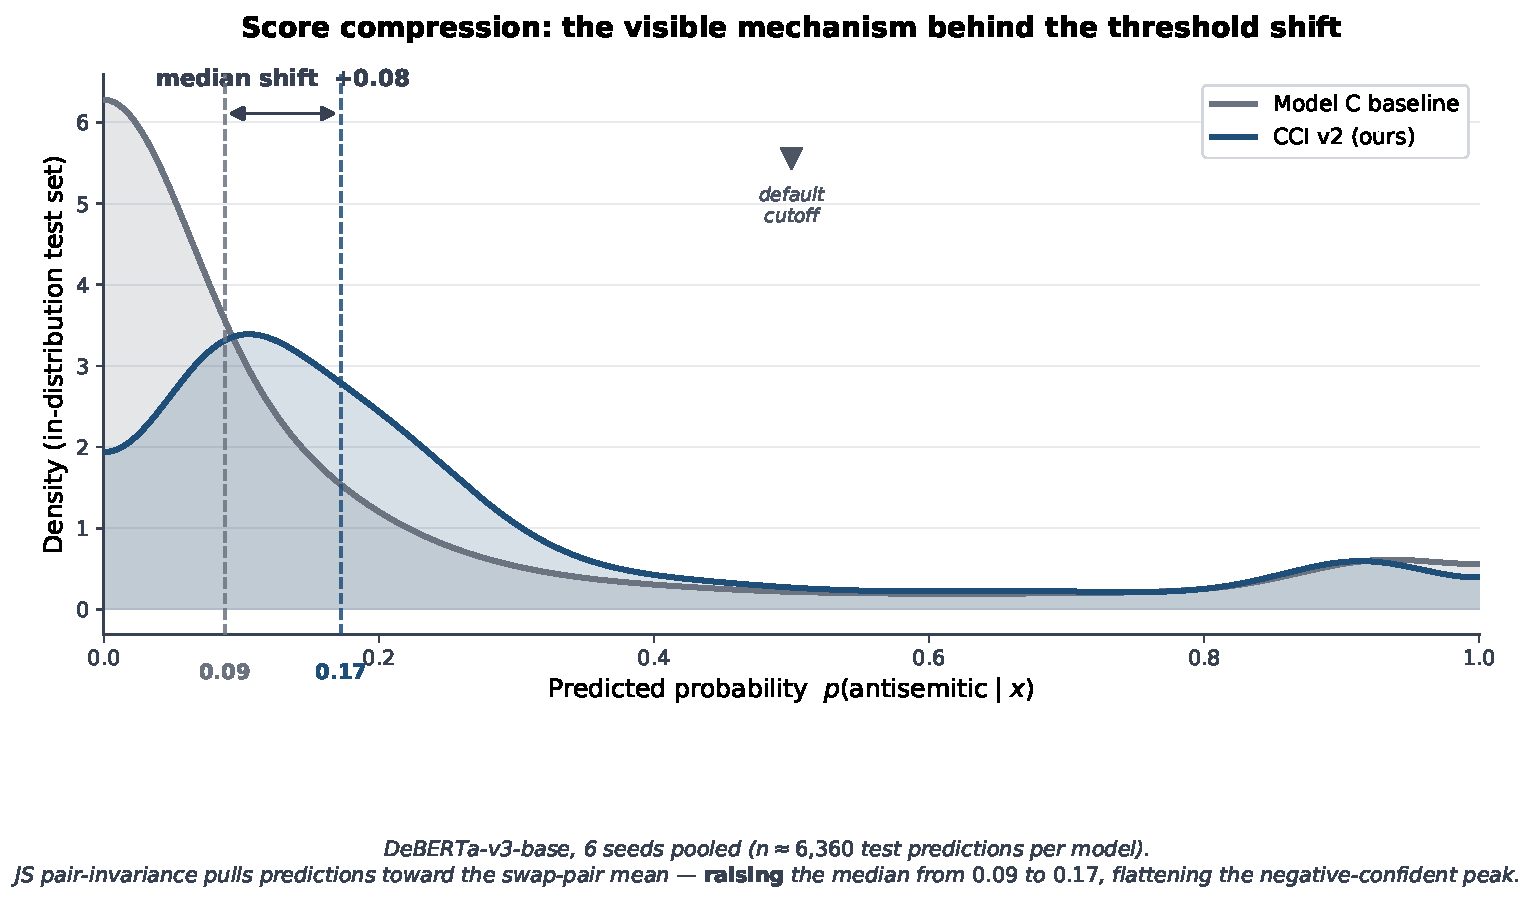
\includegraphics[width=0.95\linewidth]{../results/figures/poster_panel2_score_compression.pdf}
\caption{Score compression as the visible mechanism behind the cross-dataset threshold shift. Densities are the test-set predicted-probability distributions for Model~C (orange) and CCI~v2 (blue) on DeBERTa-v3-base, seed 42. CCI~v2's distribution is contracted toward the swap-pair mean: the right tail above 0.5 (typical of confident positive predictions) is flattened, and the bulk of probability mass sits between 0.0 and 0.2. This is the predicted behaviour of a Jensen-Shannon pair-invariance regulariser and is exactly the operating-point pattern that pushes the PR-optimal threshold from $\approx 0.5$ to $[0.05, 0.18]$ cross-dataset.}
\label{fig:panel_compression}
\end{figure}

The multi-seed sweep reports aggregate metrics only; per-keyword breakdowns shown in Table~\ref{tab:per_keyword} are therefore reported for seed 42.

\begin{table}[t]
\centering
\caption{Test-set macro-F\textsubscript{1} per keyword group (seed 42). Base rates: Jews $12.0\%$, Israel $44.6\%$, Kikes $34.8\%$, ZioNazi $8.6\%$.}
\label{tab:per_keyword}
\begin{tabular}{@{}lcccc@{}}
\toprule
\textbf{Model} & \textbf{Jews} & \textbf{Israel} & \textbf{Kikes} & \textbf{ZioNazi} \\
\midrule
A: \modelA     & 0.647 & 0.790 & 0.749 & 0.821 \\
B: \modelB     & 0.741 & 0.779 & 0.749 & \textbf{1.000} \\
B2: \modelBB   & 0.626 & 0.764 & 0.798 & 0.821 \\
C: \modelC     & \textbf{0.711} & 0.782 & 0.800 & \textbf{1.000} \\
\bottomrule
\end{tabular}
\end{table}

The ``Jews'' keyword group is the most challenging (low base rate, diverse contexts): both DeBERTa-based models outperform RoBERTa, with Model~B and Model~C showing the strongest overall performance.

\begin{figure}[h]
\centering
% \includegraphics[width=0.95\linewidth]{../results/figures/paper_fig_per_keyword.pdf}  % MISSING: generator script removed; regenerate on RCP before final build
\caption{Per-keyword macro-F\textsubscript{1} across the four GoldStandard2024 keyword groups, mean $\pm$ std over six seeds. Base rates differ by an order of magnitude (Jews 11.4\% to ZioNazi 88.3\%), so an aggregate single number can mask group-level disparities. CCI~v2 reaches the highest Jews-group F\textsubscript{1} ($0.726 \pm 0.025$), where the group is largest and the base rate is lowest, while remaining within seed noise of Model~C on Israel, Kikes, and ZioNazi. The headline aggregate gain in Table~\ref{tab:main_results} therefore tracks the hardest group rather than an easy slice; the ZioNazi group is near a ceiling for every method.}
\label{fig:per_keyword_heatmap}
\end{figure}

\subsection{Where does the model look?}
\label{sec:attribution}

To probe \emph{where} the classifier draws its signal, we compute Integrated Gradients~\citep{sundararajan2017axiomatic} attribution maps via Captum~\citep{kokhlikyan2020captum} on 500 test examples for three configurations: Model~B, the vanilla DeBERTa-v3 baseline; Model~C, which combines focal loss with identity-token masking; and CCI~v2, our counterfactual consistency model with fixed temperature and Jensen--Shannon regularization. For each example, we measure the fraction of absolute attribution mass assigned to identity tokens, using matches against identity-related stems such as \texttt{jew*}, \texttt{israel*}, \texttt{zion*}, and \texttt{kike*}. Results are aggregated across six seeds, giving 3{,}000 seed-level measurements per model.

Because the resulting attribution distribution is strongly right-skewed, we report median and interquartile range rather than mean and standard deviation. Statistical comparisons use paired Wilcoxon signed-rank tests after averaging the six seed-specific measurements for each example and model; $p$-values are Holm-corrected across the three pairwise comparisons.

\begin{table}[h]
\centering
\caption{Fraction of Integrated Gradients attribution mass assigned to identity tokens. Values are median [Q1, Q3]. Lower values indicate weaker attribution mass on identity terms. Pairwise tests are paired Wilcoxon signed-rank tests after averaging over seeds for each example.}
\label{tab:attribution}
\begin{tabular}{lccc}
\toprule
Model & Median [Q1, Q3] & $p_{\mathrm{Holm}}$ vs.\ B & $d_z$ vs.\ B \\
\midrule
Model~B (vanilla)           & 0.0532 [0.0229, 0.1121] & --- & --- \\
Model~C (focal+mask)        & 0.0465 [0.0192, 0.0994] & $6.33{\times}10^{-7}$ & 0.175 \\
CCI v2 (fixed T, JS)        & 0.0438 [0.0184, 0.0936] & $1.07{\times}10^{-12}$ & 0.270 \\
\bottomrule
\end{tabular}
\end{table}

Figure~\ref{fig:attribution} shows the full distribution of attribution mass assigned to identity tokens. Both Model~C and CCI~v2 assign less attribution mass to identity tokens than Model~B. This indicates that models trained with the focal-loss and counterfactual-consistency objectives place less salience on group identifiers than the vanilla DeBERTa baseline. CCI~v2 never sees attribution maps in its loss, so this shift is emergent rather than directly optimized.

The comparison between Model~C and CCI~v2 is statistically significant but very small ($p_{\mathrm{Holm}} = 2.98{\times}10^{-3}$, paired Wilcoxon; $d_z = 0.112$). Thus, although CCI~v2 has the lowest median and mean attribution mass, its additional reduction relative to Model~C is minor in magnitude. The larger CFR gains of CCI~v2 therefore cannot be explained by a large further reduction in token-level identity attribution alone; they are more plausibly tied to the constraint CCI~v2 places on the relative response to counterfactual pairs $(x, x')$, consistent with Lemma~\ref{thm:ts-cfr}.

\begin{figure}[h]
\centering
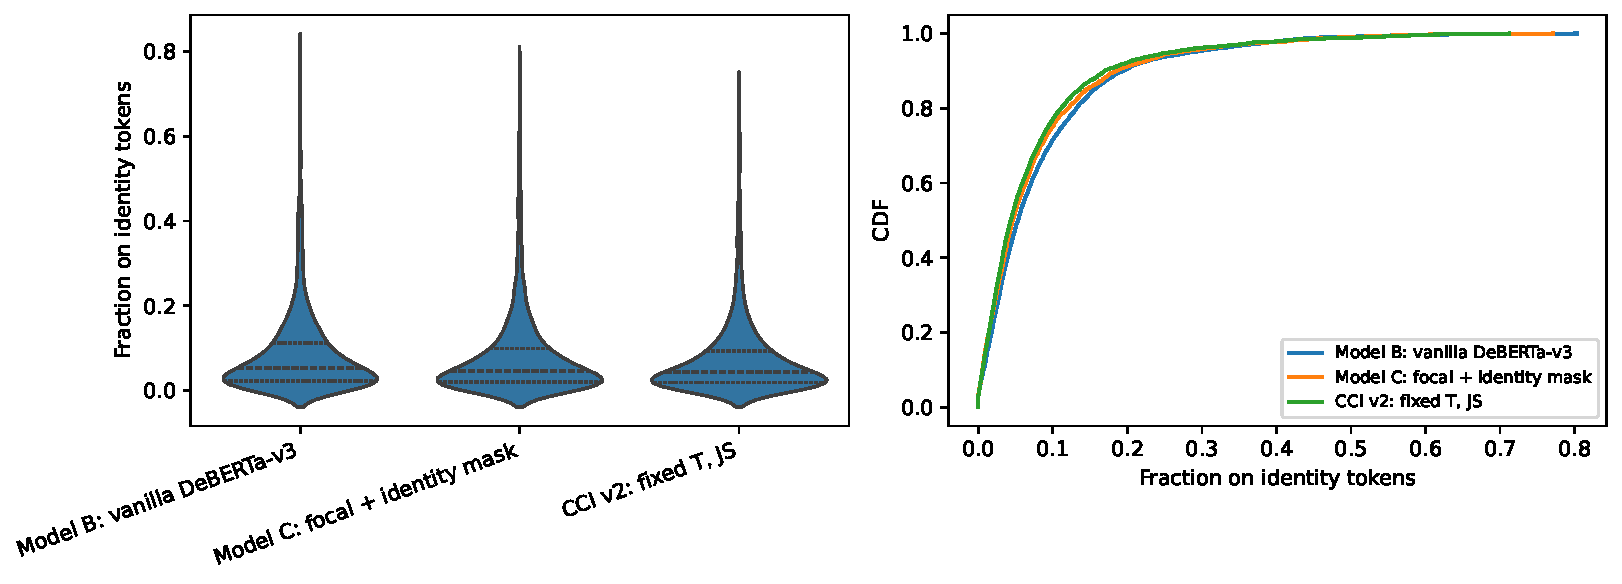
\includegraphics[width=0.85\linewidth]{figures/attribution_shift.pdf}
\caption{Distribution of the fraction of attribution mass assigned to identity tokens across 500 test examples and six random seeds. Model~C and CCI~v2 shift attribution mass away from identity tokens relative to the vanilla Model~B baseline; the additional CCI~v2 shift relative to Model~C is statistically detectable but small.}
\label{fig:attribution}
\end{figure}

\paragraph{Conditional attribution: the aggregate small effect is a directional average.}
The aggregate $d_z = 0.112$ Model~C vs.\ CCI~v2 effect averages over examples regardless of prediction outcome. Splitting by the four (true label, predicted label) outcome categories yields a substantially richer picture (Figure~\ref{fig:attribution_by_outcome}, derived from the rollup in \texttt{results/interpretability/attribution\_summary.csv}). On true-negative predictions ($n \approx 395$, the dominant class), CCI~v2 reduces identity-token attribution by $13.9\%$ relative to Model~C (median $0.045$ vs.\ $0.052$; paired Wilcoxon on the 395 examples Model~B classifies as TN: $p = 5.8 \times 10^{-6}$). On true-positive predictions ($n \approx 58$), CCI~v2 \emph{increases} identity attribution by $10.9\%$ (median $0.132$ vs.\ $0.119$). The aggregate small effect of \S\ref{sec:attribution} is therefore the unweighted average of two opposing direction-conditional dynamics. The pattern is consistent with the regulariser's intended behaviour: counterfactual invariance under identity swap is most needed in the negative class, where identity should be incidental; on actually-antisemitic content the identity group is typically the target of the hate, and attending to it is appropriate. The on-correctness conditional view therefore reinforces, rather than weakens, the pair-coupling mechanism inferred from Lemma~\ref{thm:ts-cfr}.

\begin{figure}[h]
\centering
% \includegraphics[width=0.95\linewidth]{../results/figures/paper_fig_attribution_by_outcome.pdf}  % MISSING: generator script removed; regenerate on RCP before final build
\caption{Median fraction of $|\mathrm{IG\ attribution}|$ on identity tokens, by prediction outcome, for the three models scored on the same 500-example test set (six seeds, averaged per example before category assignment). The aggregate Model~C vs.\ CCI~v2 effect ($d_z = 0.11$, Table~\ref{tab:attribution}) is the unweighted average of two opposing direction-conditional dynamics. On true-negative predictions (the dominant class, where identity should be incidental) CCI~v2 attends to identity tokens \emph{less} than Model~C ($-13.9\%$, paired Wilcoxon $p = 5.8 \times 10^{-6}$). On true-positive predictions (real antisemitism, where the identity group is typically the target of the hate) CCI~v2 attends to identity tokens \emph{more} ($+10.9\%$). The error bars are inter-quartile ranges; $n$ values along the x-axis are per-model (Model~B / Model~C / CCI~v2). The conditional view is consistent with the desired debiasing behaviour for a counterfactual-invariance loss.}
\label{fig:attribution_by_outcome}
\end{figure}

\subsection{Additional Evaluations (Pending)}

The following are part of the planned analysis and are not yet complete:

\begin{itemize}[leftmargin=*,itemsep=1pt]
  \item \textbf{LLM baselines (D1--D3).} Infrastructure is wired; pending the gated-model access token.
  \item \textbf{Keyword-sensitivity flip-rate test.} Replaces identity terms with \texttt{[MASK]} and measures prediction-change rate; expected to favour Model~C if keyword masking improved contextual (vs.\ shortcut) decisions. This diagnostic is complementary to the Integrated Gradients analysis in \S\ref{sec:attribution}: Integrated Gradients measures gradient-based token salience on the original input, whereas the keyword-sensitivity flip-rate test measures whether masking identity terms changes the model's discrete prediction.
  \item \textbf{Cross-dataset transfer.} Zero-shot application of the best checkpoint to HateXplain and ToxiGen, as per the methodology.
  \item \textbf{Temporal robustness.} Train-era vs.\ post-2022 split of the test set.
\end{itemize}

